\documentclass[a4paper, 11pt]{article}
\usepackage[utf8]{inputenc}
\usepackage{float}
\usepackage{graphicx}
\usepackage{url}
\usepackage{enumitem}
\usepackage{subcaption}

\setlist[itemize]{itemsep=0.5pt, parsep=0.5pt, topsep=0pt, partopsep=0pt}
\setlist[enumerate]{itemsep=0.5pt, parsep=0.5pt, topsep=0pt, partopsep=0pt}

%opening
\title{HW3 Report, Loggy: A Logical Time Logger}
\author{David Fischer}
\date{\today{}}

\begin{document}

\maketitle

\section{Introduction}
Lamport and vector clocks serve as fundamental tools that enable causal ordering in distributed systems. Though implementations might differ, their core principles are still represented in multiple areas such as distributed tracing, message queues, and distributed garbage collection.
This assignment's goal was the implementation of \textit{Loggy}, a logging procedure continually receiving and logging messages from workers.

The implementation spans a central logging module with a holdback queue to print ordered messages, workers sending and receiving messages between each other on a random delay with random jitters before reporting to the central logger, two clock modules, Lamport and vector based, and analytics modules to generate insights.

\section{Implementation}

\subsection{Time}

% DONE: explain time module in my own words
The Lamport \textit{time} module contains functions to initialize, update, and review timestamps and clocks.
The Lamport implementation handles timestamps as simple numbers and the clock as a map which contains the worker names keys and individual timestamps as values.
Updating the clock is handled by comparing the current value with the new value from the specified process and then changing the map if the new value is greater.
A message is determined as safe to print when the given timestamp is less or equal to the minimum value from the clock map.

The same methodology was applied to the vector (\textit{vect}) module, with the major difference being individual timestamps functioning like the clock from the Lamport implementation. This also makes the \texttt{safe/2} function equivalent to the \texttt{leq/2} function, as identifying whether a message with a vector timestamp is safe to log is done by checking if the timestamp is causally before or concurrent with the current clock state.

To use both modules without changes to the workers or \textit{Loggy}, requiring recompilation, the \texttt{apply/3} function was utilized.

\subsection{Holdback Queue}

The holdback queue in the \textit{Loggy} module was implemented as a simple list, starting out empty initially.
Each time a message is received, it is appended to the holdback queue, which is then sorted using the \texttt{time:leq/2} function.
The sorted list is then split with \texttt{lists:partition/2} calling \texttt{time:safe/2} using the clock held by the loop and the timestamp from each message in the queue.
The resulting entries in the \texttt{Safe} list are then logged and the \texttt{Unsafe} list is passed to the next recursive function call of \texttt{loggy:loop/3}.

% from assignment: How do we know if messages are safe to print?
% What is it that the final log tells us? Did events happen in the order presented by the log? 

\section{Main problems and solutions}

\subsection{Validating Order}

Confirming the order of messages printed by \textit{Loggy} presented a challenge initially, as issues could be caused by the clock and holdback queue implementation. Additionally, insight into the clock state and real-time messages of each individual process was limited. 
A jitter value set to \texttt{0} results in the holdback queue being skipped completely and messages being printed in order instantly when received. This output was then cross-checked with a regular test run, the numbers and delays being the same, as the randomness of the workers is seeded.
To further confirm order, even with jitters greater than zero and especially for the vector clock, a \textit{mermaid} state chart graphing module was created as an observability tool. 

\subsection{Log Parsing}
% difficulty reading the log until the log output was made clean using the built in padding
Once the vector clock module was implemented mentally parsing the \textit{Loggy} output posed a greater challenge.
To ease the load, control sequences were utilized to format the logged messages in a more coherent and readable way.

\begin{verbatim}
io:format("log: s:~-2w ~-6s ~-8w (~3w) c:~w~n", [:]).
log: s:0  george sending ( 99) c:john => 5,paul => 8,ringo => 6
\end{verbatim}

\section{Evaluation}

% Do some tests and identify situations where log entries are printed in the wrong order. 
% DONE: How do you identify messages that are in the wrong order?
% What is always true, and what is sometimes true? How do you play it safe?

\subsection{Truths}

With this implementation, one can state that causal ordering is always preserved and therefore always true due to the individual timestamps shared by the workers and the implementation of the holdback queue.
The \texttt{safe/2} function guarantees correctness, as it ensures a message is only printed when no earlier timestamp could arrive. 
To aid evaluating this, the module \textit{mermaid} creates visual representations of the messages flowing between the workers including the data and clock states. Examples of these visualizations and corresponding \textit{Loggy} outputs can be found in the Appendix.

It is sometimes true that the logged ordering exactly matches the real-time ordering. This is due to the artificial jitters in communication with \textit{Loggy}, occurring in situations where events are concurrent, like two independent workers sending a message.

\subsection{Queue Size Comparison}

\begin{figure}[H]
  \begin{center}
    \begin{subfigure}[b]{0.494\textwidth}
      \centering
      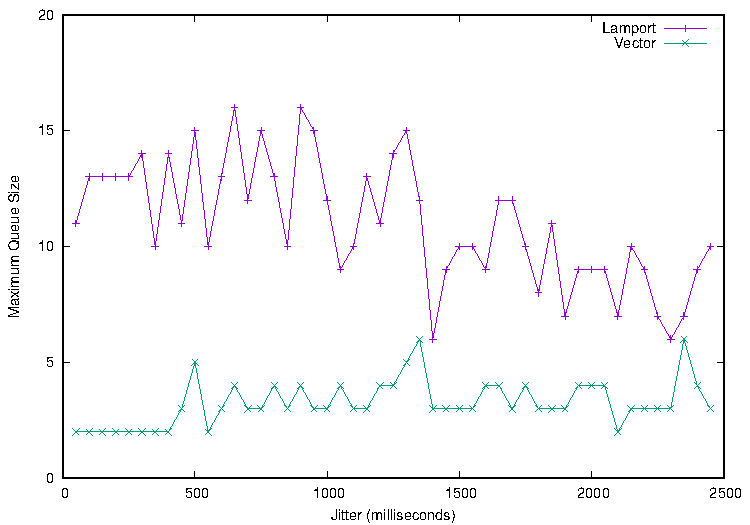
\includegraphics[width=\textwidth]{test/jitter.pdf}
      \caption{Jitter with 1500ms \texttt{Sleep}}
      \label{fig:results1}
    \end{subfigure}
    \hfill
    \begin{subfigure}[b]{0.494\textwidth}
      \centering
      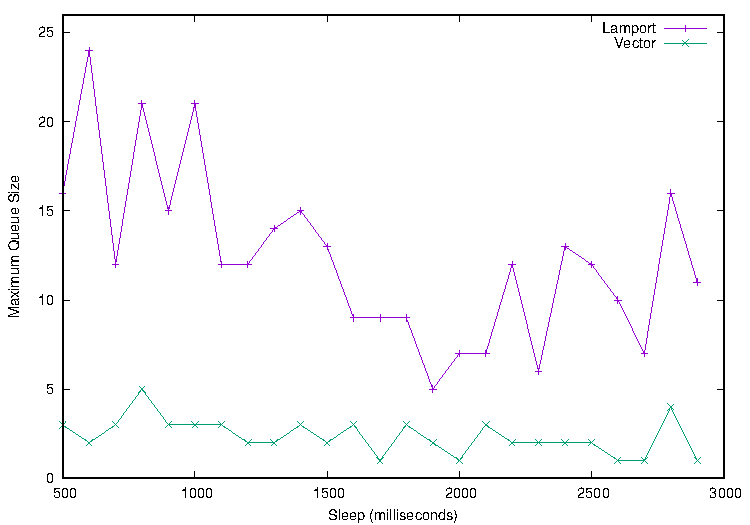
\includegraphics[width=\textwidth]{test/sleep.pdf}
      \caption{Sleep with 250ms \texttt{Jitter}}
      \label{fig:results2}
    \end{subfigure}
  \end{center}
  \caption{Queue size comparison on different delays and jitters}
  \label{fig:comparison}
\end{figure}

Due to the inherent randomness of the \textit{Loggy} implementation these results can't be taken as absolutes for correlating sleep or jitter to the maximum queue size.
Still, the difference between the maximum size of the Lamport queue when compared to the vector queue demonstrates the logging throughput being greater, at the cost of larger messages.

Also notable is the bypass of the holdback queue when the \texttt{Jitter} is set to zero as can be seen in Figure \ref{fig:results1}.
% actually validate that the queue size isn't too big, logging seems weird right now, 
% CONFIRMED: i'm just stupid the queue size is always printed by all the same logging outs

\section{Conclusions}

In conclusion, the holdback queue is crucial to maintain causal order to guarantee \textit{sends} being logged before \textit{receives}, although it cannot guarantee correctness for independent concurrent events. 
Improvements to the current implementation include replacing \texttt{apply/3} with a shared time module to improve performance, as it will always be slower than direct function calls, and implementation of more sophisticated observability as the current \textit{mermaid} module can't correctly represent concurrent \textit{send} messages.

\newpage

\appendix

\section{Lamport Clock}
These tests were completed using \texttt{test:run(<module>, 1500, 500).}

\begin{verbatim}
119> test:run(time, 1500, 500).
loggy: starting with module time
log: s:5   ringo  sending  ( 24) c:1
log: s:5   john   sending  (  6) c:1
log: s:5   george sending  ( 26) c:1
log: s:2   paul   received ( 24) c:2
log: s:2   john   received ( 26) c:2
log: s:2   paul   received (  6) c:3
log: s:2   john   sending  ( 50) c:3
log: s:2   ringo  received ( 50) c:4
log: s:2   john   sending  ( 73) c:4
log: s:2   paul   sending  ( 28) c:4
log: s:8   george received ( 28) c:5
log: s:8   ringo  sending  (  2) c:5
log: s:8   john   sending  ( 37) c:5
log: s:13  george received ( 73) c:6
log: s:13  paul   received (  2) c:6
log: s:13  john   sending  (  1) c:6
log: s:3   george sending  ( 48) c:7
log: s:3   paul   sending  ( 30) c:7
log: s:3   ringo  received ( 48) c:8
log: s:3   paul   received ( 37) c:8
log: s:3   ringo  sending  ( 86) c:9
log: s:3   george received ( 86) c:10
log: s:3   george received ( 30) c:11
log: s:3   george sending  ( 85) c:12
log: s:3   ringo  received ( 85) c:13
log: s:3   ringo  sending  ( 83) c:14
log: s:3   george received ( 83) c:15
log: s:3   ringo  received (  1) c:15
\end{verbatim}
% \caption{Test execution of the lamport clock}

\begin{figure}[H]
  \begin{center}
    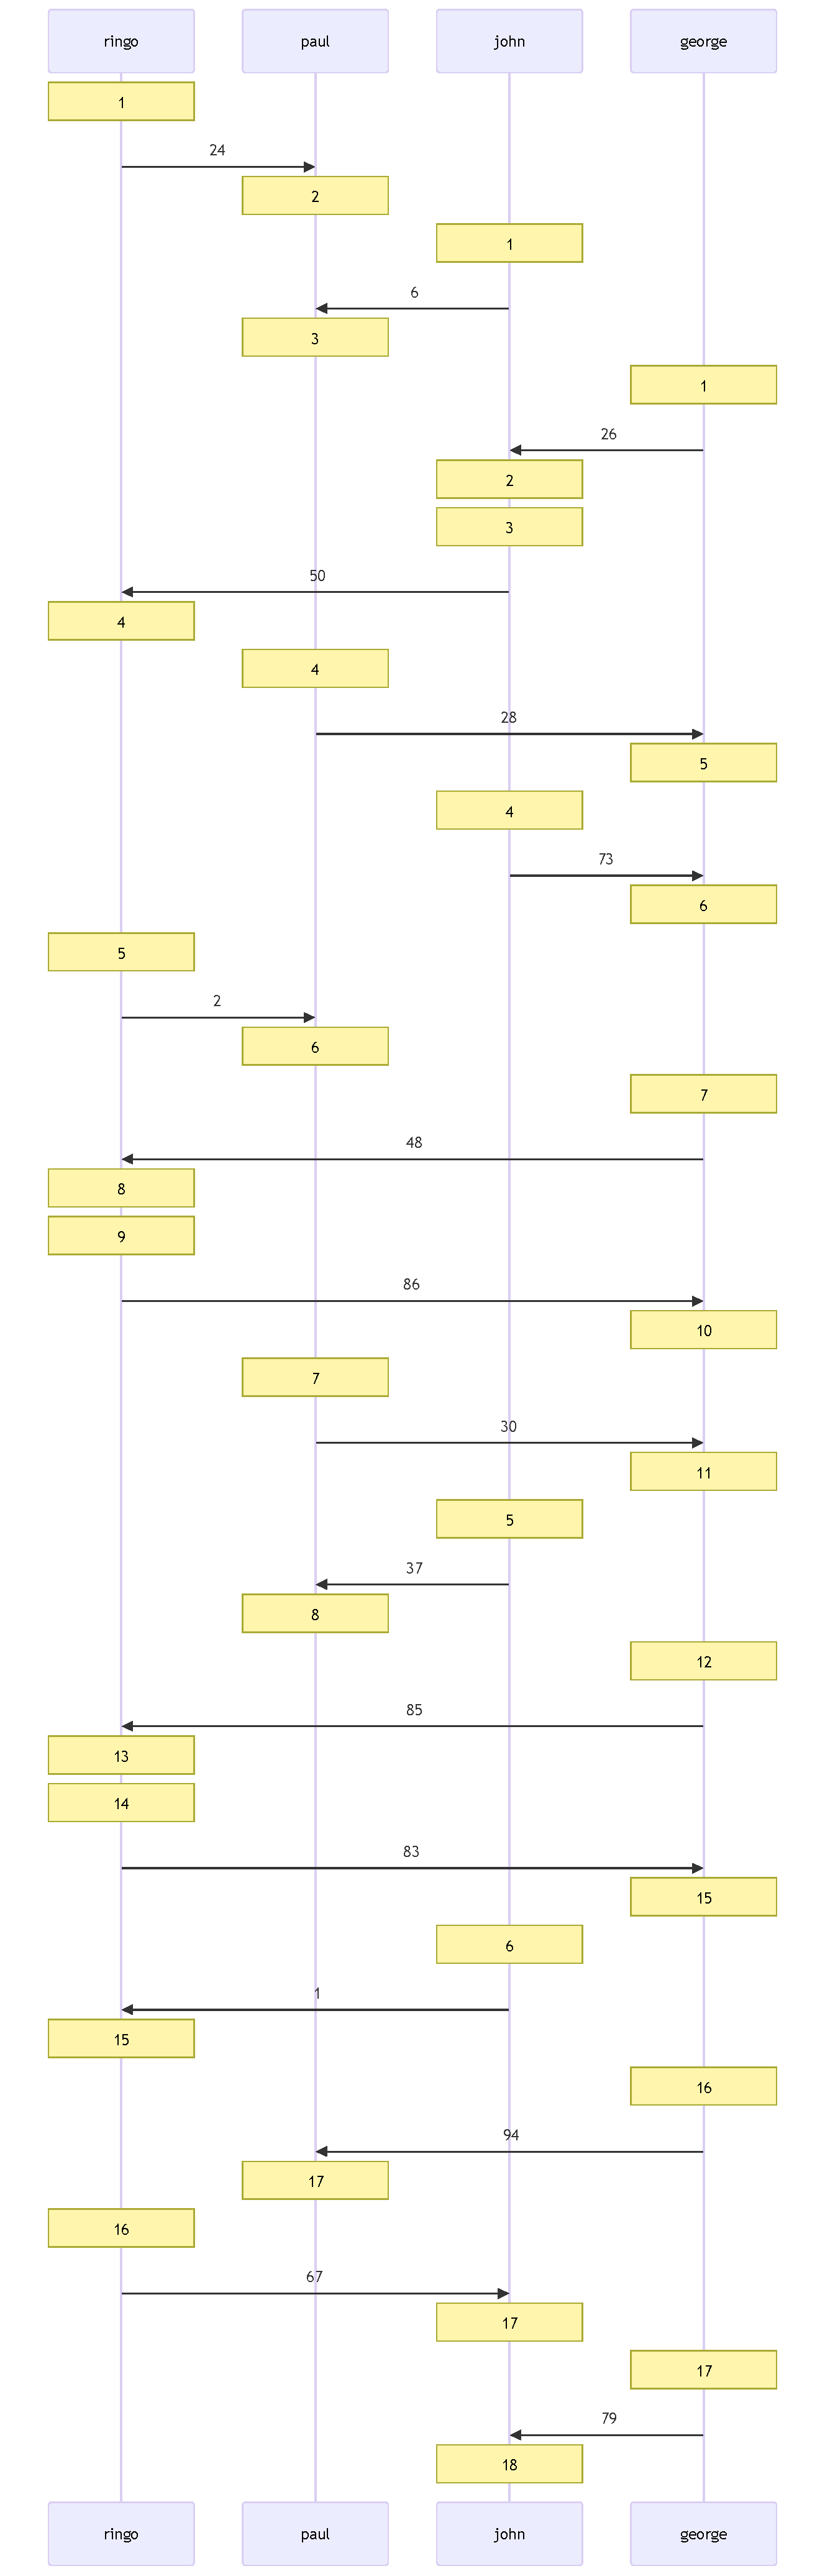
\includegraphics[height=0.985\textheight]{graphics/mermaid_lamport.pdf}
    \caption{Sequence visualization of the Lamport timestamp algorithm}
    \label{fig:seq1}
  \end{center}
\end{figure}

\section{Vector Clock}
\begin{verbatim}
120> test:run(vect, 1500, 500).
loggy: starting with module vect
log: s:1   ringo  sending  ( 24) c:ringo => 1
log: s:1   paul   received ( 24) c:paul => 1,ringo => 1
log: s:0   john   sending  (  6) c:john => 1
log: s:0   paul   received (  6) c:john => 1,paul => 2,ringo => 1
log: s:0   george sending  ( 26) c:george => 1
log: s:0   john   received ( 26) c:john => 2,george => 1
log: s:0   john   sending  ( 50) c:john => 3,george => 1
log: s:0   ringo  received ( 50) c:john => 3,ringo => 2,george => 1
log: s:2   john   sending  ( 73) c:john => 4,george => 1
log: s:0   paul   sending  ( 28) c:john => 1,paul => 3,ringo => 1
log: s:0   george received ( 28) c:john => 1,paul => 3,ringo => 1,george => 2
log: s:0   george received ( 73) c:john => 4,paul => 3,ringo => 1,george => 3
log: s:0   ringo  sending  (  2) c:john => 3,ringo => 3,george => 1
log: s:0   paul   received (  2) c:john => 3,paul => 4,ringo => 3,george => 1
log: s:0   george sending  ( 48) c:john => 4,paul => 3,ringo => 1,george => 4
log: s:0   ringo  received ( 48) c:john => 4,paul => 3,ringo => 4,george => 4
log: s:1   john   sending  ( 37) c:john => 5,george => 1
log: s:1   paul   received ( 37) c:john => 5,paul => 5,ringo => 3,george => 1
log: s:0   ringo  sending  ( 86) c:john => 4,paul => 3,ringo => 5,george => 4
log: s:0   george received ( 86) c:john => 4,paul => 3,ringo => 5,george => 5
log: s:2   george sending  (  8) c:john => 4,paul => 3,ringo => 5,george => 6
log: s:1   ringo  sending  ( 84) c:john => 4,paul => 3,ringo => 6,george => 4
log: s:1   paul   received ( 84) c:john => 5,paul => 6,ringo => 6,george => 4
log: s:1   paul   received (  8) c:john => 5,paul => 7,ringo => 6,george => 6
log: s:1   paul   sending  ( 46) c:john => 5,paul => 8,ringo => 6,george => 6
log: s:1   george received ( 46) c:john => 5,paul => 8,ringo => 6,george => 7
log: s:1   john   sending  (  1) c:john => 6,george => 1
log: s:1   ringo  received (  1) c:john => 6,paul => 3,ringo => 7,george => 4
log: s:0   george sending  ( 99) c:john => 5,paul => 8,ringo => 6,george => 8
log: s:0   paul   received ( 99) c:john => 5,paul => 9,ringo => 6,george => 8
\end{verbatim}

\begin{figure}[H]
  \begin{center}
    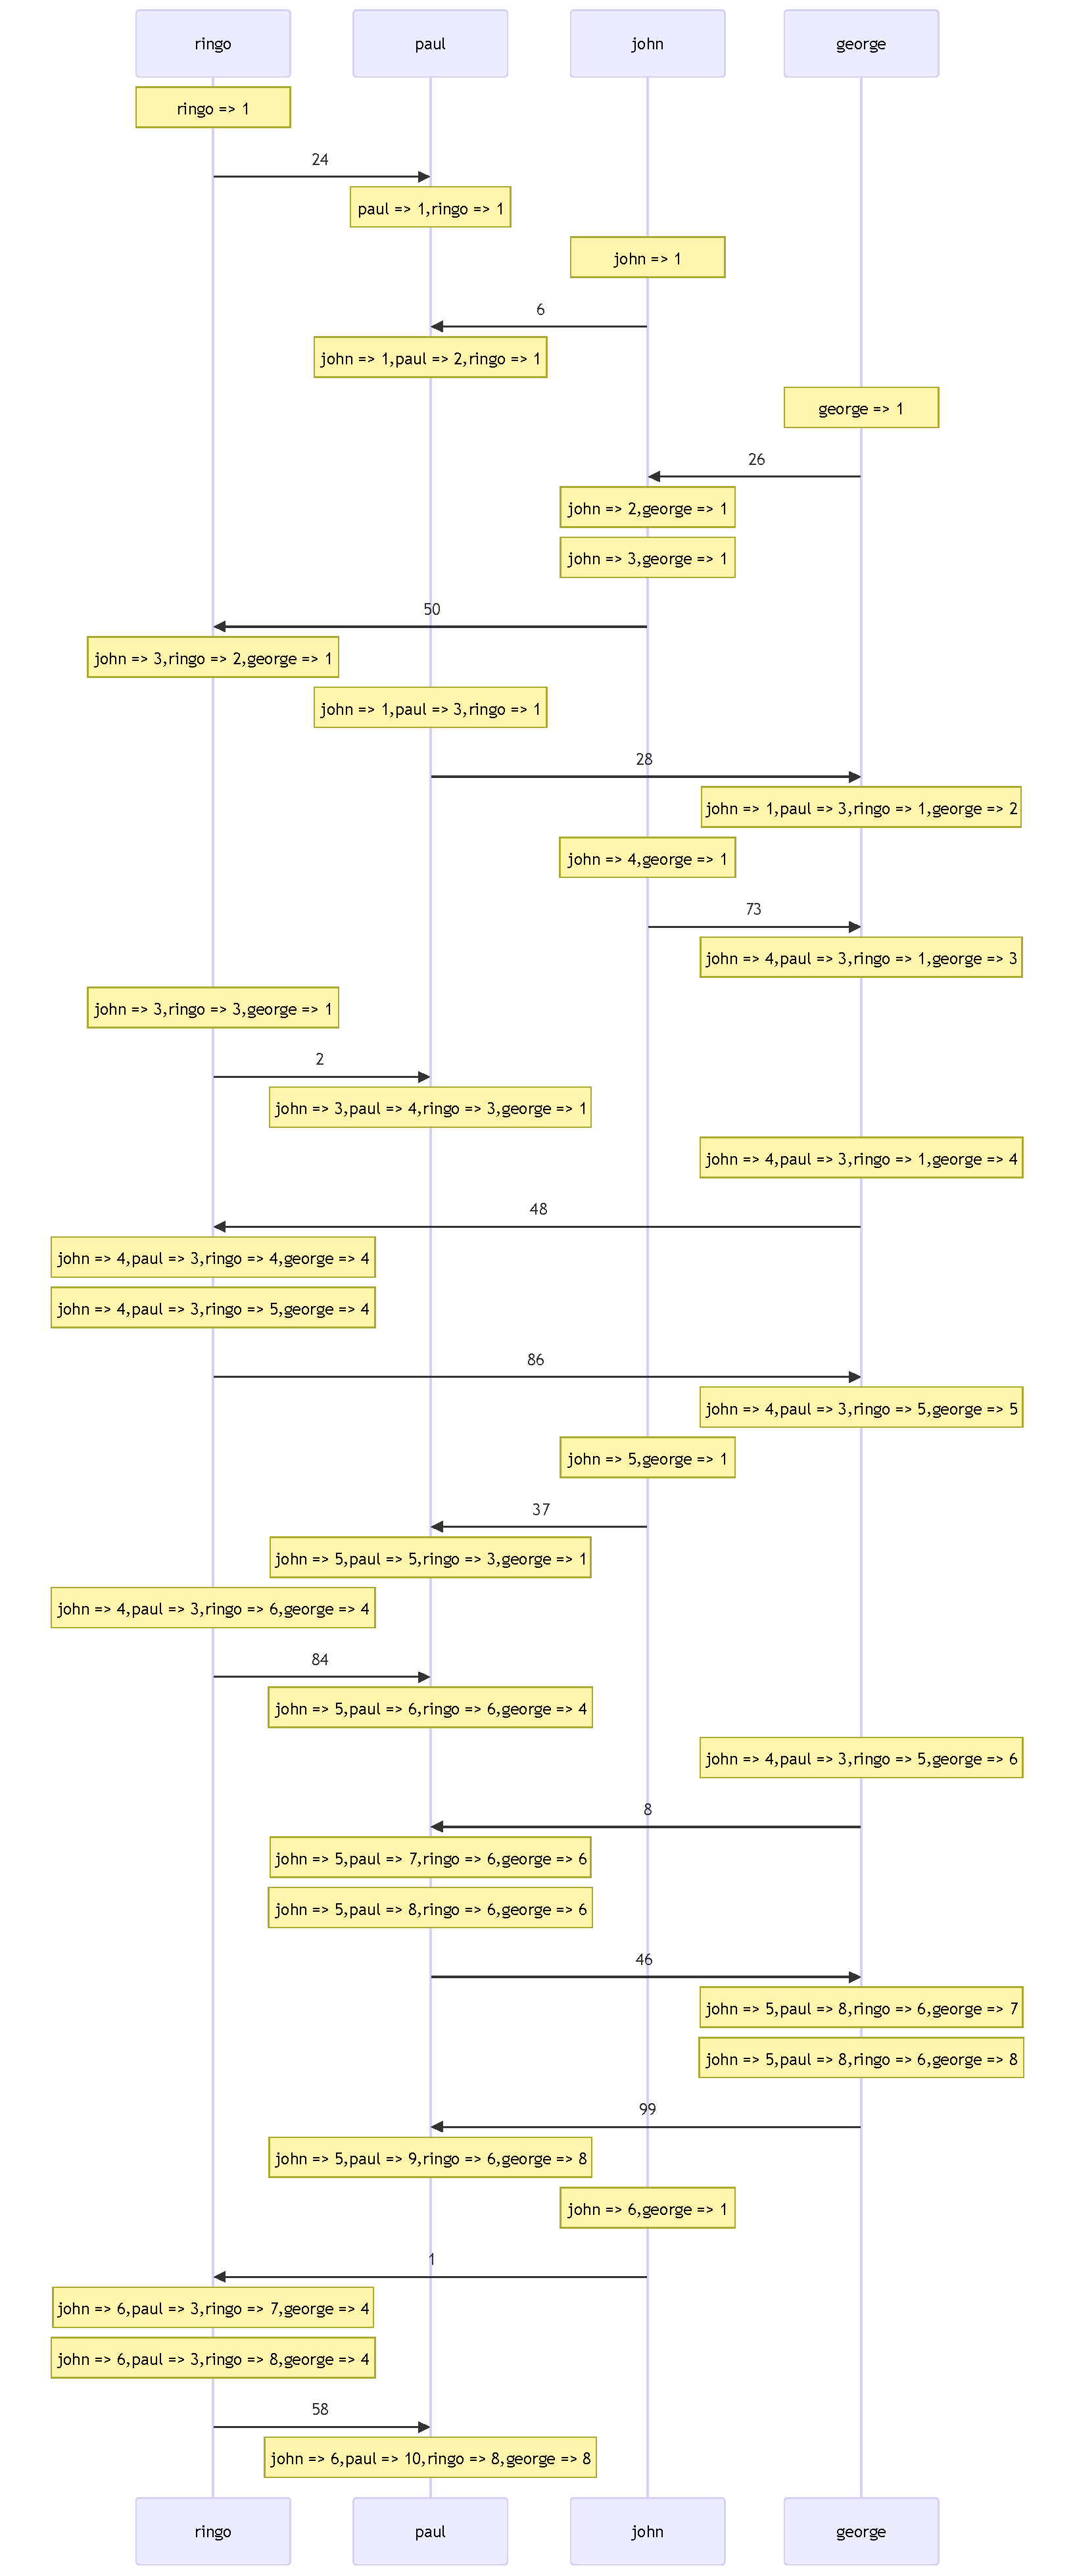
\includegraphics[height=0.985\textheight]{graphics/mermaid_vector.pdf}
    \caption{Sequence visualization of the vector clock implementation}
    \label{fig:seq2}
  \end{center}
\end{figure}

\end{document}
